\documentclass{article}%
\usepackage[T1]{fontenc}%
\usepackage[utf8]{inputenc}%
\usepackage{lmodern}%
\usepackage{textcomp}%
\usepackage{lastpage}%
\usepackage{authblk}%
\usepackage{graphicx}%
%
\title{Pharmacokinetics of Naja sumatrana (Equatorial Spitting Cobra) Venom and Its Major Toxins in Experimentally Envenomed Rabbits}%
\author{Richard Thompson}%
\affil{Department of Molecular and Human Genetics, Baylor College of Medicine, Houston, Texas, United States of America}%
\date{01{-}01{-}2012}%
%
\begin{document}%
\normalsize%
\maketitle%
\section{Abstract}%
\label{sec:Abstract}%
SAN DIEGO {-} A new study shows that brain and eye disease that results from mutant kidney cells in mice has an association with blood{-}borne susceptibility to antibody{-}mediated autoimmune disorders such as psoriasis, diabetes and lupus.\newline%
Previous studies have shown that diseases associated with antibody{-}mediated autoimmune disorders can also lead to inflammatory conditions that are characterized by inflammation associated with the disease system. The findings indicate that exposures to immune cell{-}associated potentially infectious agents have an association with blood{-}borne engebrances and disease mechanisms.\newline%
Targeting the nervous system and immune systems for inflammatory and immune{-}related diseases may support the developing of targeted therapeutics tailored for these diseases said Birgit Wenzel, M.D., vice president of research and clinical development at Ithaca University.\newline%
In this study, the researchers identified a single gene, VirB9{-}1, that is significant for the highly invasive chronic beta{-}thalassemia. VirB9{-}1 is a hallmark of type IV and non{-}intravenous beta{-}thalassemia, which are mainly diagnosed in adults with the rare blood condition.\newline%
The researchers discovered VirB9{-}1 in blood samples from diabetic mice, as well as from healthy control mice. The VirB9{-}1 gene was found in both other and normal beta{-}thalassemia patients. In non{-}diabetic diabetic mice, VirB9{-}1 was also found in tissues belonging to immune system cells involved in infection and inflammatory responses.\newline%
This is a positive evidence{-}based discovery of this gene in Type IV alpha{-}thalassemia and should expedite the development of therapeutic strategies that target this gene, Dr. Wenzel said.\newline%
We also demonstrated in other mouse models that VirB9{-}1 may affect the insulin{-}producing beta{-}thalassemia and may be able to boost good insulin function, Dr. Wenzel added.\newline%
Data provided at the publication by Ithaca University is available on the FDA{-}regulated website at www.FDA.gov . The subjects were tested in a coma facility at the U.S. National Institutes of Health (NIH) in Bethesda, Md. Participants had their blood drawn to study exposure to VirB9{-}1 and VirB10, expressed in blood circulating through the intestine. The most common disease characteristics in diabetic mice were autoimmune conditions, diabetes and psoriasis.\newline%
In January 2013, FDA released a draft EU Clinical Publication Quality Directive (CQDP) approval of investigational nucleoside analogues, nucleoside prophylactic therapies and nucleoside antisense analogues based on the VirB9{-}1 gene expressing.\newline%
In 2011, the FDA published a pathway for diagnosing, monitoring and appropriate prescribing the VirB9{-}1 gene expressing blood in these and other tests. Based on data from the CQDP study, this pathway was expanded in 2012 to include blood type testing.\newline%
\#\#\#

%
\subsection{Image Analysis}%
\label{subsec:ImageAnalysis}%


\begin{figure}[h!]%
\centering%
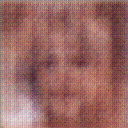
\includegraphics[width=150px]{500_fake_images/samples_5_355.png}%
\caption{A Close Up Of A Black And White Photo Of A Zebra}%
\end{figure}

%
\end{document}